\begin{savequote}[75mm]
This is a really enlightening quote. 
\qauthor{Tomo Lazovich}
\end{savequote}

\chapter{Combined limits from boosted and resolved searches}
\label{chap:4bcomb}

\section{Introduction}

In order to cover the full mass range of possible resonances decaying to di-Higgs final states, two distinct tailored selections were produced. The resolved selection is more sensitive in the mass range of $400 < m_{X} < 1100 \GeV$ while the boosted selection is more sensitive to masses in the range $1100 < m_{X} < 3000 \GeV$. Chapter 7 presents the details of the boosted selection and results. In setting limits on spin-2 Randall-Sundrum graviton (RSG) and narrow width heavy scalar ($H$) models, the results of the boosted selection are combined with the results of the resolved selection to cover the full mass range.

This chapter presents limits on signal models resulting from the $\FourBfull$ search in both the resolved and boosted selections. It first presents a brief overview of the resolved results that go into the limit setting. Then, an overview of the statistical methods used for the search and limit setting is given. Finally, limits on the RSG and heavy scaler models are presented. 

\section{Resolved results}

The details of the resolved selection will not be presented here and can be found in reference~\cite{4bconf}. In basic terms, the selection searches for four $R = 0.4$ b-tagged calorimeter jets (where each pair of jets is one Higgs candidate). This is distinct from the boosted methodology which searches for merged decay products. The backgrounds to the resolved selection are the same as those presented in Chapter 7 for the boosted analysis. 

Table~\ref{tab:ResolvedResults} shows the results for data yields and expected background in the resolved signal region. Figure~\ref{fig:ResolvedResults} shows the $M_{2J}$ distribution in the resolved signal region. The total number of events is consistent with the prediction and no significant excess is seen. One event in the boosted $4$-tag signal is shared with the resolved signal region and has a mass of $852 \GeV$. 

\begin{table}[!ht]
\begin{center}
\begin{tabular}{ l c  }
\toprule
 Sample      & Signal Region Yield \\ 
\midrule
Multijet     & $43.3 \pm 2.3$   \\
$\ttbar$       &  $4.3 \pm 3.0$   \\
%$Z$+jets     &  < 0.2           \\
$Z$+jets     &  -           \\
\midrule
Total        & $47.6 \pm 3.8$   \\
 \midrule
Data         & $46$    \\
\midrule
SM $hh$ & $0.25 \pm 0.07$ \\
$\Gkk$$\left(800\,\rm{\GeV}\right)$, $c = 1$ & $5.7 \pm 1.5$ \\
\bottomrule
\end{tabular}
\caption{Observed yields in the resolve selection $4$-tag signal region compared to the predicted number of background events
  Errors correspond to the total uncertainties in the predicted event yields. The yields for a graviton with $m_{\Gkk} = 800\GeV$ and $c = 1$ are also shown.~\cite{4bconf}}
\label{tab:ResolvedResults} 
\end{center}
\end{table}

\begin{figure}[h!]
  %\vspace{20pt}
  \centering
  \captionsetup{justification=centering}

  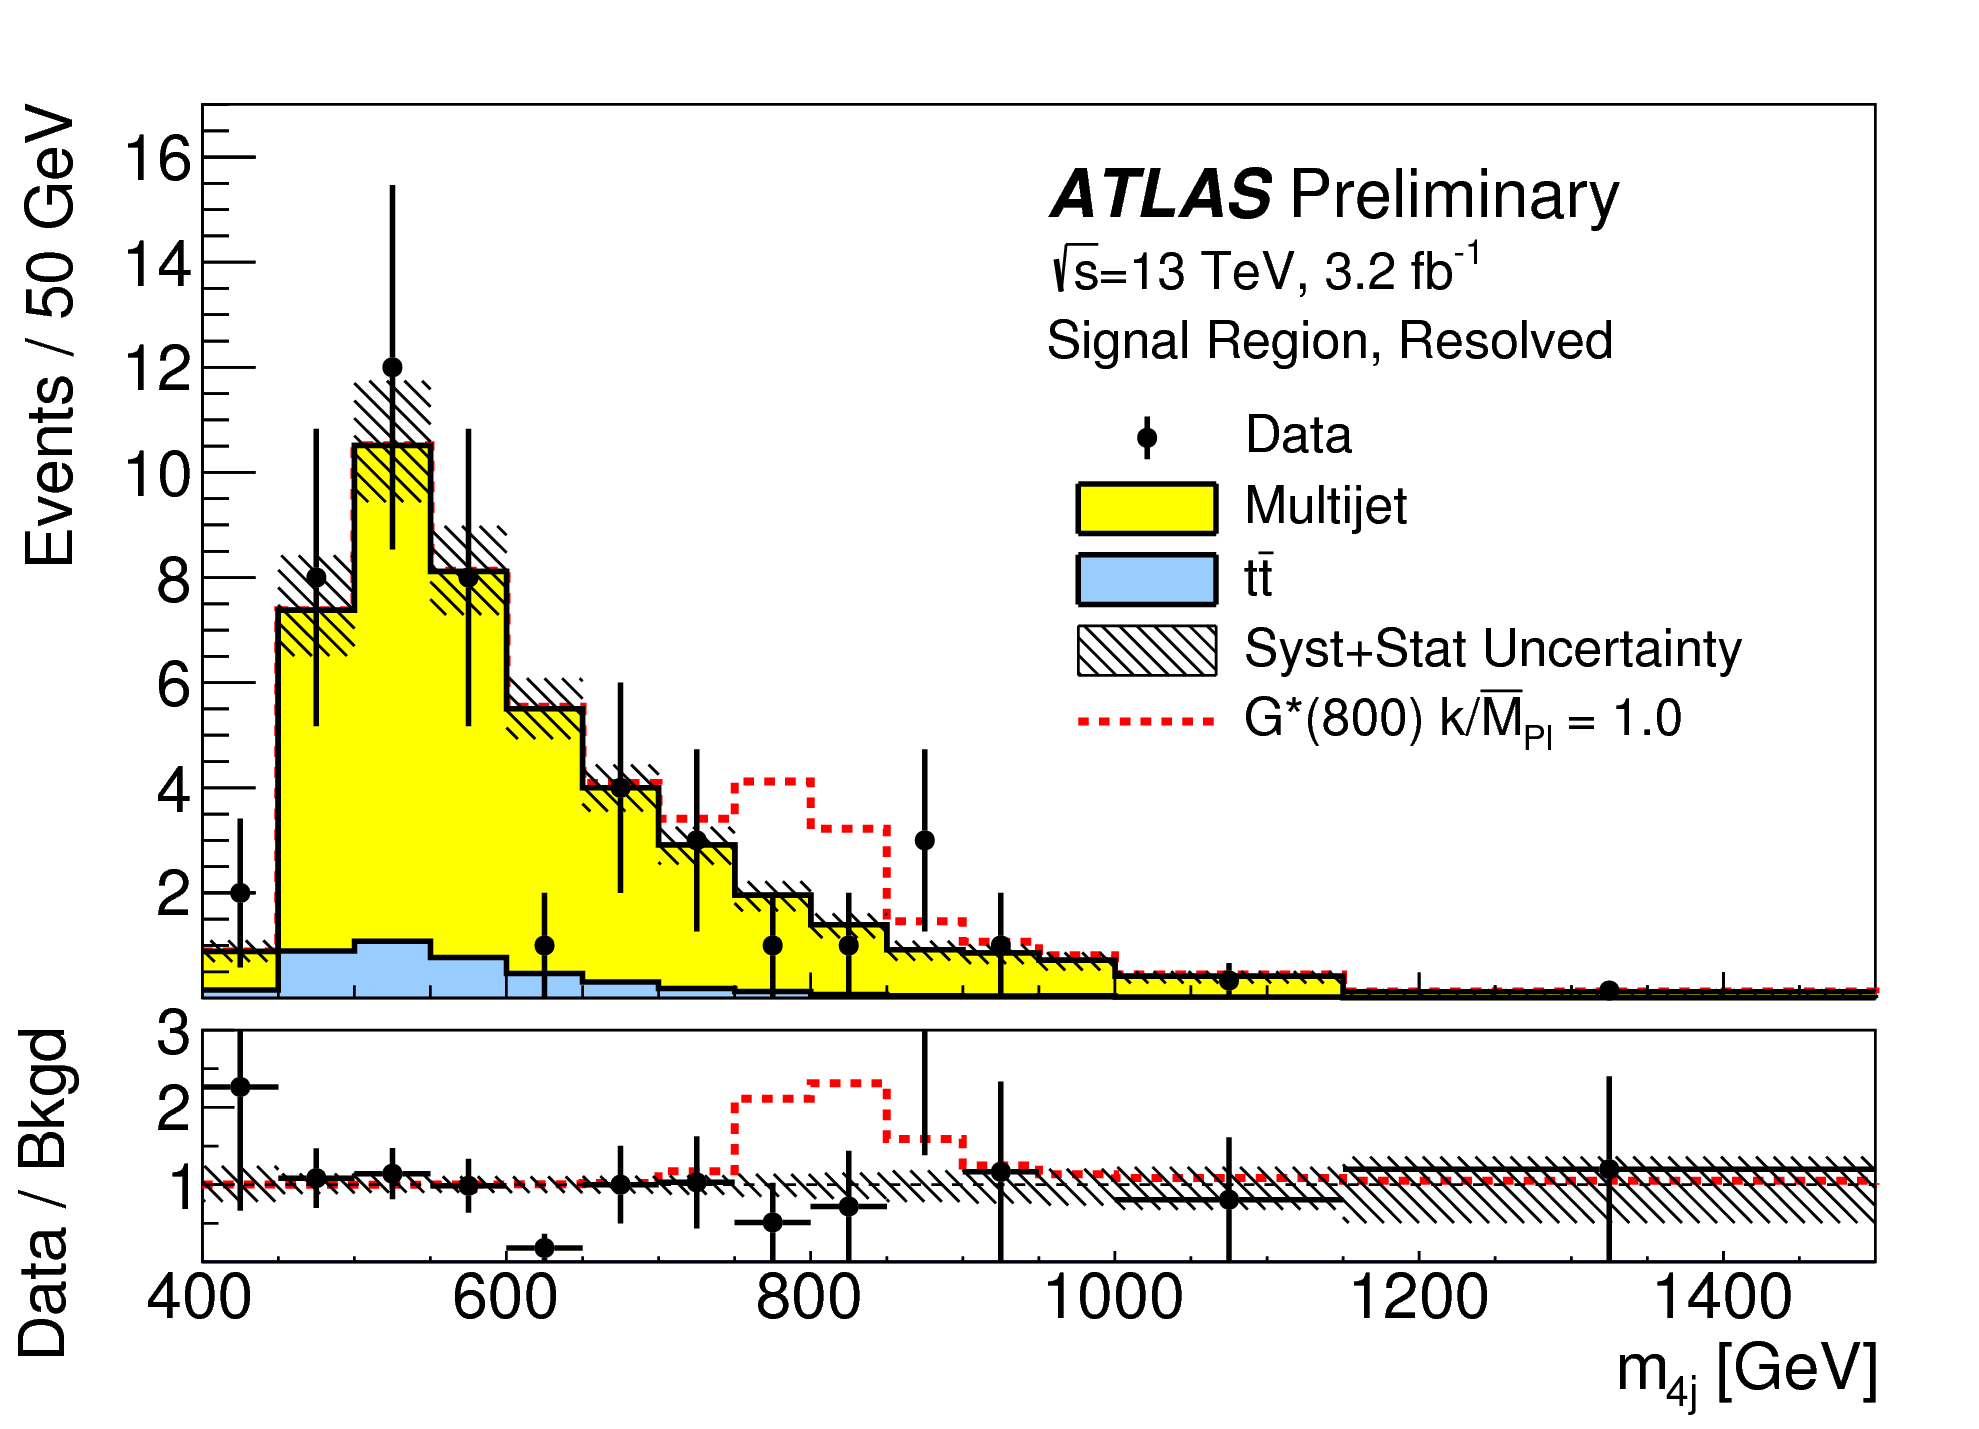
\includegraphics[width=0.6\textwidth]{figures/Resolved_signal}


   \caption{Di-jet invariant mass ($M_{2J}$) in the resolved signal region. A graviton signal with $m_{\Gkk} = 800 \GeV$ and $c=1$ is overlaid. ~\cite{4bconf}.}
  \label{fig:ResolvedResults}
\end{figure}

\section{Search technique and results}

The statistical technique used for the search in this analysis is the same as that used in the $\HWW$ analysis presented in section~\ref{sec:ww_stats}. The test statistic $q_0$ is used to define the $p$-values which measure the compatibility of the data with the background-only hypothesis corresponding to a signal strength $\mu = 0$. 

Local $p_0$ values are computed to quantify the probability that the background could produce a fluctuation greater than or equal to the one observed in the data. In the resolved analysis, no significant excesses are observed. The largest discrepancy with respect to the background only hypothesis occurs near a resonance mass of $900 \GeV$ and is found to be less than $2\sigma$ in significance.

In the boosted selection, the largest local excess is a broad excess in the $3b$ signal region that begins near $M_{2J} \approx 1.7 \GeV$. Assuming a $\Gkk$ with this mass and $c=1.0$, the local significance of this excess is $2.0 \sigma$. 

\section{Limit setting}

In the absence of any significant excess observed in the data, limits on different signal models can be set. This section describes the limit setting procedure and presents combined results of the resolved and boosted analyses. 

\subsection{Limit setting procedure}

The procedure used for setting exclusion limits in this analysis is the CL$_{s}$ method~\cite{CLS}. The first step in setting the limits is to define a test statistic which will be used. For limit setting, the test statistic is shown in equation~\ref{eqn:4b_limit_q}. 
%
\begin{equation}
\label{eqn:4b_limit_q}
  \widetilde{q_{\mu}} =
  \begin{cases}
    -2\ln \frac{L(\mu,\hat{\hat{\theta}}(\mu))}{L(0,\hat{\hat{\theta}}(0))} & \hat{\mu} < 0 \\
    -2\ln \frac{L(\mu,\hat{\hat{\theta}}(\mu))}{L(\hat{\mu},\hat{\theta})} & 0 \le \hat{\mu} < \mu \\
    0 & \hat{\mu} > \mu
  \end{cases} 
\end{equation}
%
In the above equation, $\mu$ is the value of the signal strength under test, $\hat{mu}$ is the best fit $\mu$, $\hat{theta}$ is the best fit value of the nuisance parameters, $\hat{\hat{\theta}}$ is the best fit value of the nuisance parameters under the fixed $\mu$ value, and $L$ is the Poisson likelihood of the data (as described in section~\ref{sec:ww_stats}). 

The test statistic $\widetilde{q_{\mu}}$ is constructed to protect against two interesting corner cases when setting the upper limit on the cross section. First, it protects against negative signal strengths $\mu$ which are unphysical. Second, it does not count excesses in the data larger than those expected by a signal strength $\mu$ as evidence against the $\mu$ hypothesis. 

The CL$_{s}$ statistic is constructed by taking a ratio of two probabilities. CL$_{s+b}$ is the probability that the signal+background hypothesis would produce a value of the test statistic that is less than or equal to the observed value\footnote{Lower values of $\widetilde{q_{\mu}}$ mean better compatibility}. CL$_{b}$ is the probability that the that the background only hypothesis will produce a value of the test statistics less than or equal to the observed. The CL$_{s}$ statistic is then the ratio CL$_{s+b}$/CL$_{b}$. A $95\%$ upper limit on the cross section is set at the value of $\mu$ that makes the CL$_{s}$ statistic less than $5\%$. 

In practice, the limits are computed numerically within an asymptotic approximation for the distribution of the test statistic $\widetilde{q_{\mu}}$. The details of this approximation can be found in reference~\cite{Cowan:2010st}. 

The resolved and boosted analyses are combined using a very simple procedure rather than a full statistical combination. For each mass point tested, the limit which gives the most stringent constraint is used. This means that for mass points below $1.1 \TeV$ the resolved signal region is used, while at and above this point the combination of the orthogonal $3b$ and $4b$ boosted signal regions is used. 

\subsection{Limit setting results}

Figure~\ref{fig:4b_limits} shows the combined $95\%$ upper bounds as a function of mass for three different models: $\Gkk$ with $c=1$, $\Gkk$ with $c=2$, and a narrow heavy scalar $H$. 

\begin{figure}[!ht]
\centering
\captionsetup{justification=centering}

    \begin{subfigure}[t]{\textwidth}
        \centering
        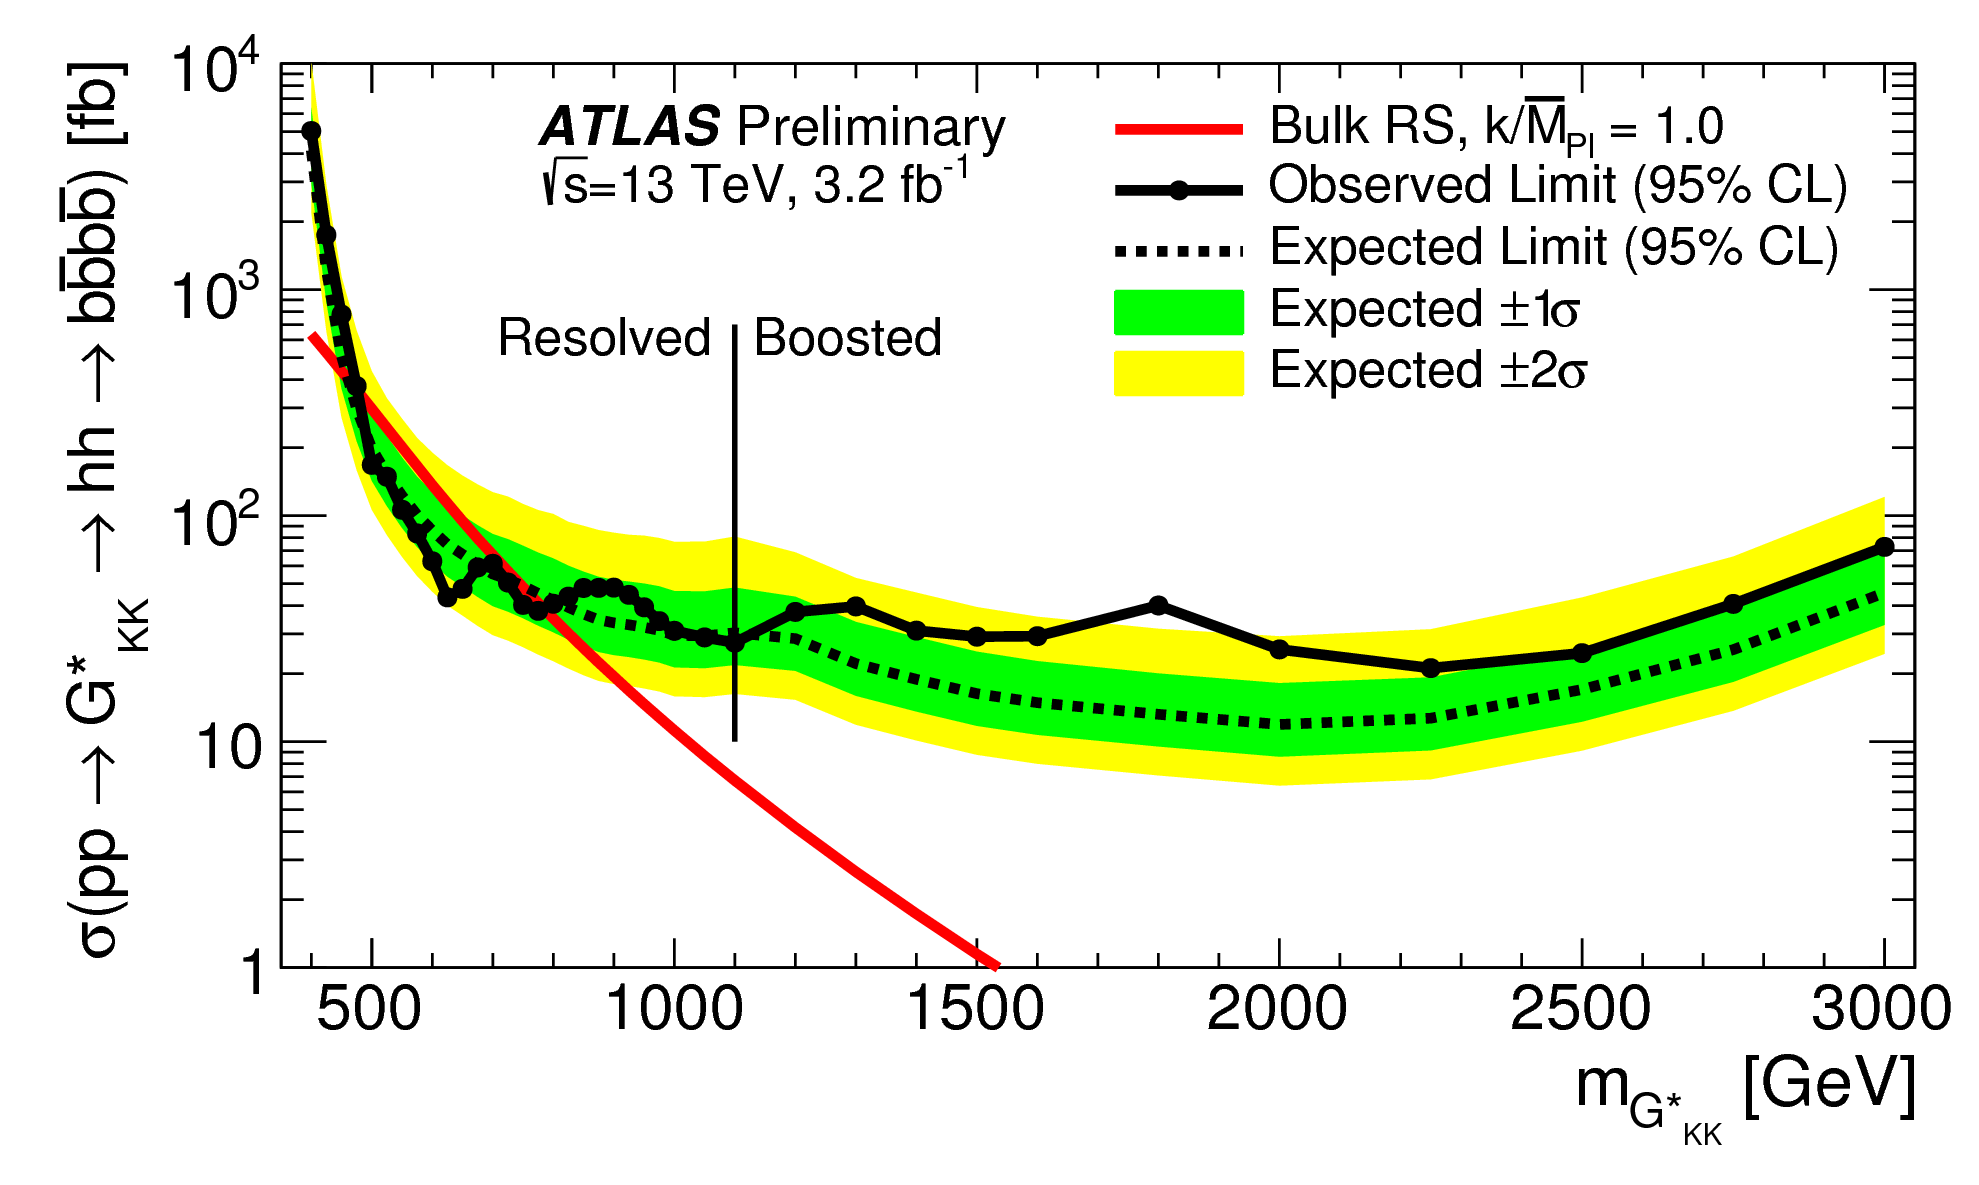
\includegraphics[width=0.7\textwidth]{figures/Limit_RSG_c1}
        \caption{Bulk RS, $c = 1$}
    \end{subfigure}%

    \begin{subfigure}[t]{\textwidth}
        \centering
        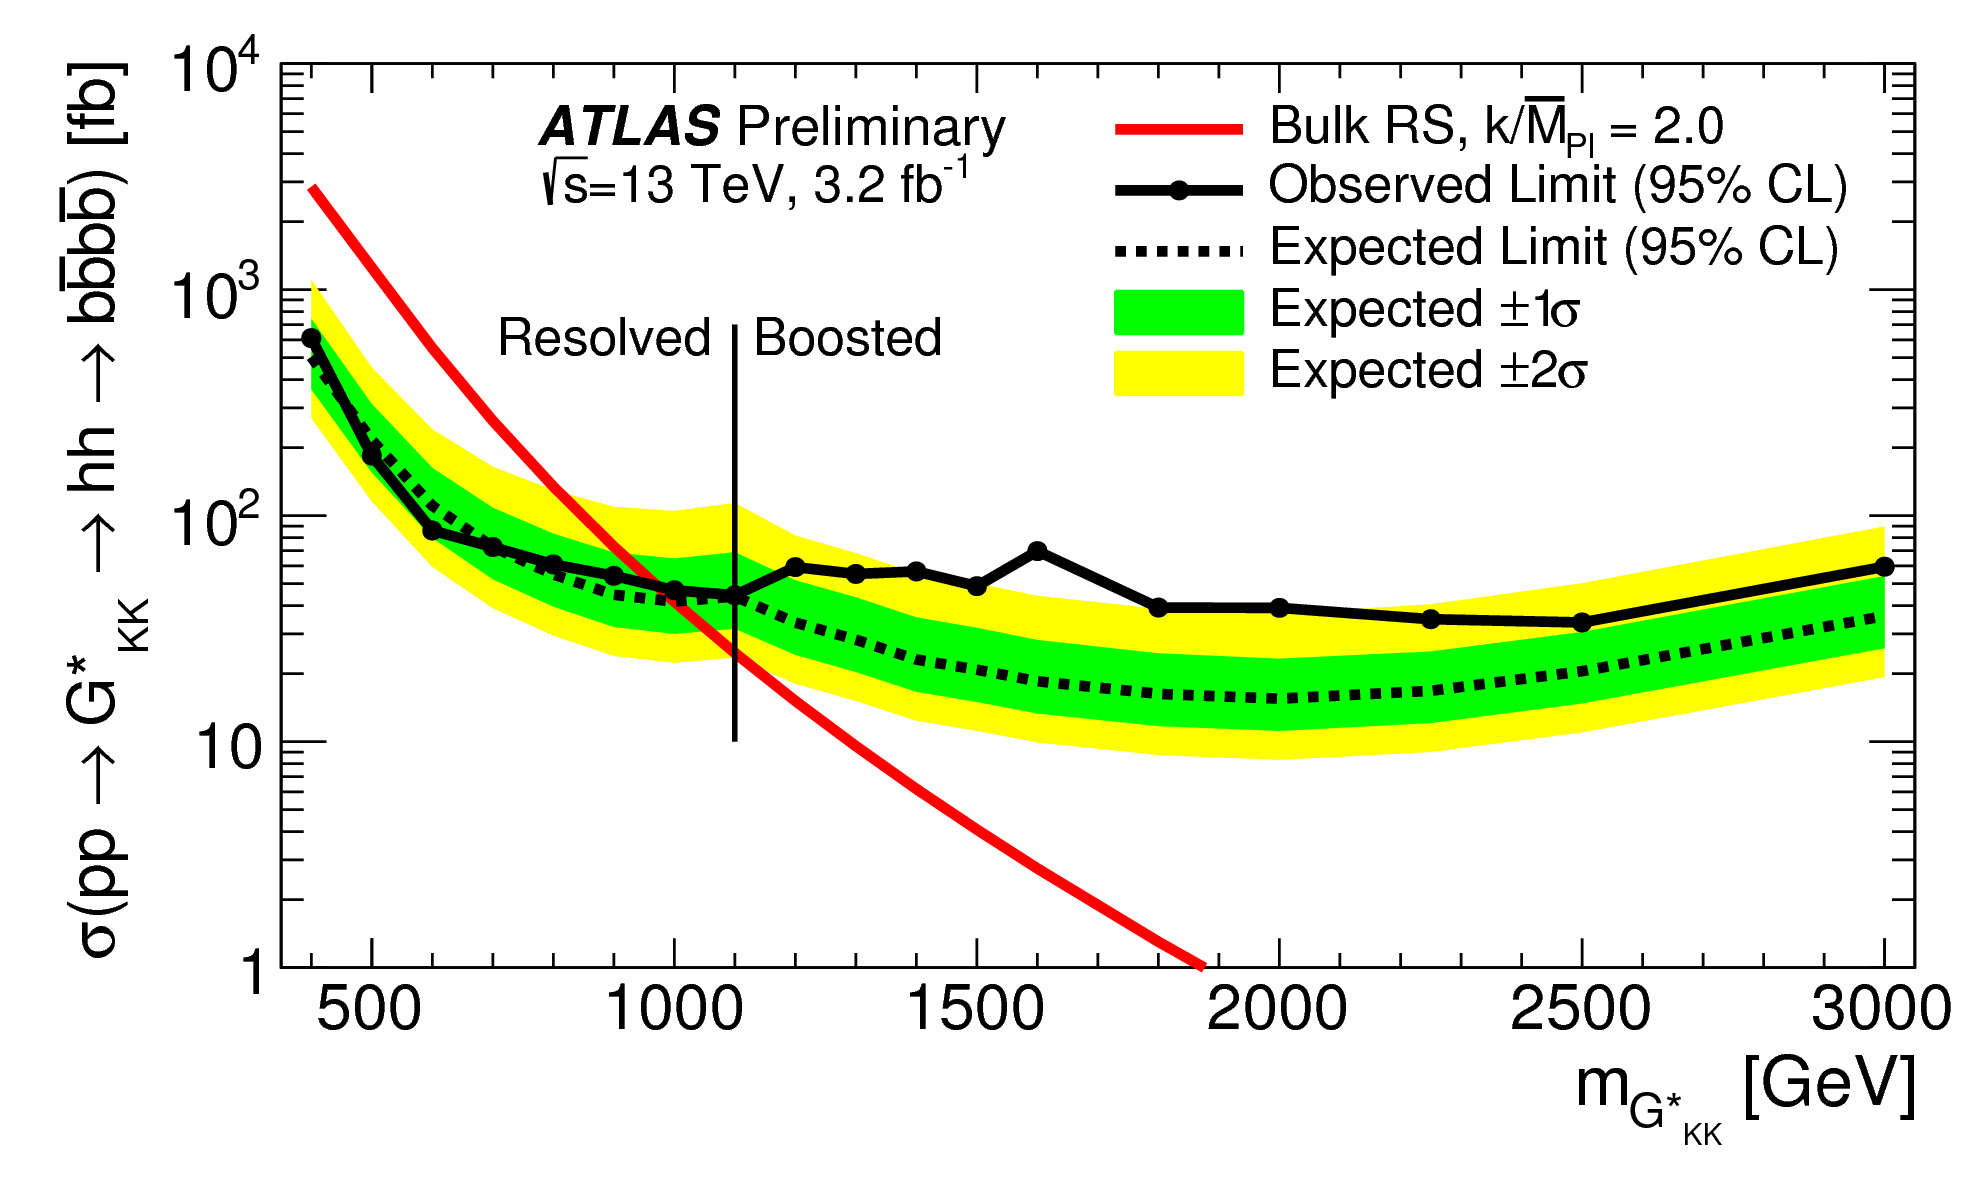
\includegraphics[width=0.7\textwidth]{figures/Limit_RSG_c2}
        \caption{Bulk RS, $c = 2$}
    \end{subfigure}%

    \begin{subfigure}[t]{\textwidth}
        \centering
        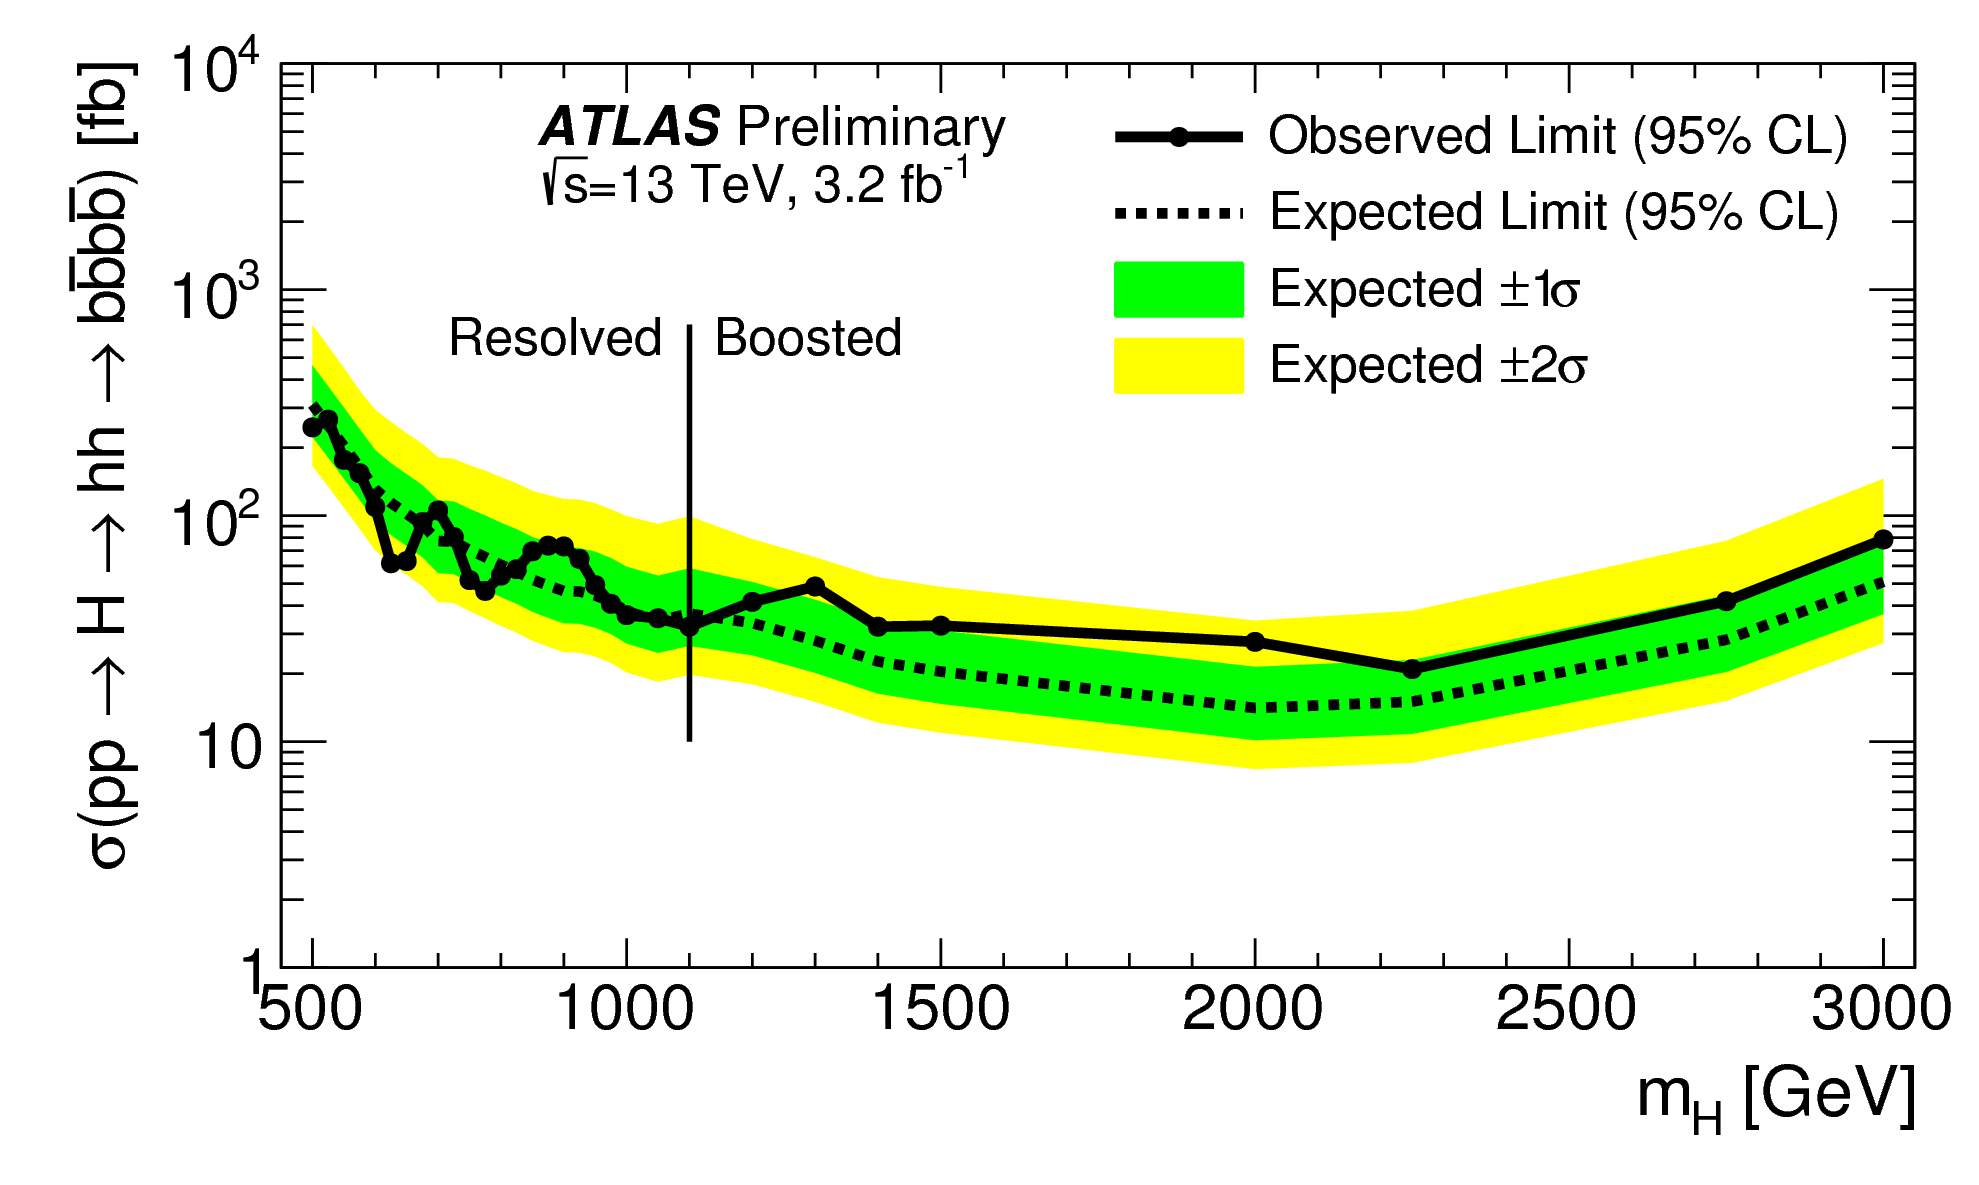
\includegraphics[width=0.7\textwidth]{figures/Limit_H}
        \caption{Spin-0 narrow-width $H$ boson}
    \end{subfigure}%
\caption{Expected and observed upper limit as a function of mass for $\Gkk$ in the RSG model with (a) $c = 1$
  and (b) $c = 2$, as well as (c) $H$ with fixed $\Gamma_H = 1\,\GeV{}$, at the 95\% confidence level in the CL$_{s}$ method.~\cite{4bconf}}
\label{fig:4b_limits}
\end{figure}

The cross section of $\sigma(pp \to \Gkk \to hh \to b\bar{b}b\bar{b})$ with $c=1$ is constrained to be less than $70 \fb$ for masses in the range $600 < m_{\Gkk} < 3000 \GeV$. For the RSG model with $c=2$, cross sections limits between $40\fb$ and $200 \fb$ are set for the mass range of $500 < m_{\Gkk} < 3000 \GeV$. Masses in the range of $475 < m_{\Gkk} < 785 \GeV$ are excluded with $c=1$ (with an exclusion of the range $465$ to $745 \GeV$ expected). Masses less than $980 \GeV$ are excluded with $c=2$ (with an exclusion for masses less than $1 \TeV$ expected). 

In the heavy Higgs model, the cross section upper limits for $\sigma(pp \to H \to hh \to b\bar{b}b\bar{b})$ ranges from $30$ to $300 \fb$ in the mass range of $500 < m_{H} < 3000 \GeV$. 
%
The resolved analysis can also set an upper limit on the Standard Model di-Higgs production cross section discussed in chapter 3. The upper limit on $\sigma(pp \to hh \to b\bar{b}b\bar{b})$ in the Standard Model is constrained to be less than $1.22 \pb$. 


